\section{Usability test}
In the following sections are shown the results of the previous sections aggregated making the average of the values for each different user profile:

\subsection{Profile 1}
\begin{table}[H]
  \begin{center}
    \begin{tabular}{||c|c|c|c|c|c||} % <-- Alignments: 1st column left, 2nd middle and 3rd right, with vertical lines in between
      \textbf{Scenario} & \textbf{Task} & \textbf{Time Execution} & \textbf{Effectiveness} & \textbf{Error} & \textbf{Satisfaction}\\
      
      \hline
        1 & 1 & 11.6 & 1.0 & 0 & 5\\
        1 & 2 & 8 & 1.0 & 0 & 5\\
        1 & 3 & 15.4 & 1.0 & 0 & 5\\
        1 & 4 & 8.8 & 1.0 & 0 & 5\\
        1 & 5 & 37.6 & 1.0 & 0 & 5\\
        1 & 6 & 17 & 1.0 & 0.2 & 3.8\\
        \hline
        2 & 1 & 8.8 & 1.0 & 0 & 4.8\\
        2 & 2 & 16.4 & 1.0 & 0 & 5\\
        2 & 3 & 29.6 & 1.0 & 0 & 5\\
        2 & 4 & 8.6 & 1.0 & 0 & 4.6\\
        \hline
        3 & 1 & 10.6 & 1.0 & 0 & 5\\
        3 & 2 & 22.8 & 1.0 & 0 & 4.8\\
        3 & 3 & 32.2 & 1.0 & 0 & 5\\
        \hline

    \end{tabular}
  \end{center}
  \caption{Average results of Profile 1}
\end{table}

\subsection{Profile 2}


\begin{table}[H]
  \begin{center}
    \begin{tabular}{||c|c|c|c|c|c||} % <-- Alignments: 1st column left, 2nd middle and 3rd right, with vertical lines in between
      \textbf{Scenario} & \textbf{Task} & \textbf{Time Execution} & \textbf{Effectiveness} & \textbf{Error} & \textbf{Satisfaction}\\
      
      \hline
        1 & 1 & 25 & 1.0 & 0 & 3.8\\
        1 & 2 & 9.6 & 1.0 & 0 & 4.6\\
        1 & 3 & 30.2 & 1.0 & 0.4 & 4.6\\
        1 & 4 & 6.4 & 1.0 & 0 & 4.8\\
        1 & 5 & 34.6 & 1.0 & 0 & 4.8\\
        1 & 6 & 42.25 & 1.0 & 0.2 & 4.2\\
        \hline
        2 & 1 & 13.8 & 1.0 & 0 & 4.8\\
        2 & 2 & 28.2 & 1.0 & 0 & 4.4\\
        2 & 3 & 28.8 & 1.0 & 0.6 & 4.6\\
        2 & 4 & 34.5 & 0.6 & 0.6 & 3.8\\
        \hline
        3 & 1 & 18.2 & 1.0 & 0 & 4.6\\
        3 & 2 & 30.4 & 1.0 & 0 & 4.6\\
        3 & 3 & 40.4 & 1.0 & 0 & 4.4\\
        \hline

    \end{tabular}
  \end{center}
  \caption{Average results of Profile 2}
\end{table}

\subsection{Total Average}

\begin{table}[H]
  \begin{center}
    \begin{tabular}{||c|c|c|c|c|c||} % <-- Alignments: 1st column left, 2nd middle and 3rd right, with vertical lines in between
      \textbf{Scenario} & \textbf{Task} & \textbf{Time Execution} & \textbf{Effectiveness} & \textbf{Error} & \textbf{Satisfaction}\\
      
      \hline
        1 & 1 & 18.3 & 1.0 & 0 & 4.4\\
        1 & 2 & 8.8 & 1.0 & 0 & 4.8\\
        1 & 3 & 22.8 & 1.0 & 0.2 & 4.8\\
        1 & 4 & 7.6 & 1.0 & 0 & 4.9\\
        1 & 5 & 36.1 & 1.0 & 0 & 4.9\\
        1 & 6 & 29.625 & 1.0 & 0.2 & 4\\
        \hline
        2 & 1 & 11.3 & 1.0 & 0 & 4.8\\
        2 & 2 & 22.3 & 1.0 & 0 & 4.7\\
        2 & 3 & 29.2 & 1.0 & 0.3 & 4.8\\
        2 & 4 & 21.55 & 0.8 & 0.3 & 4.2\\
        \hline
        3 & 1 & 14.4 & 1.0 & 0 & 4.8\\
        3 & 2 & 26.6 & 1.0 & 0 & 4.7\\
        3 & 3 & 36.3 & 1.0 & 0 & 4.7\\
        \hline

    \end{tabular}
  \end{center}
  \caption{Average results for Profiles 1+2}
\end{table}

\bigskip

\begin{figure}[H]
  \centering
  \makebox[\linewidth]{
    
\includegraphics[scale=0.35]{images/averages.png}
    }
    \caption{Average of the results along each variable.}
\end{figure}
\bigskip
\subsection{Survey results}
\bigskip
\begin{figure}[H]
  \centering
  \makebox[\linewidth]{
    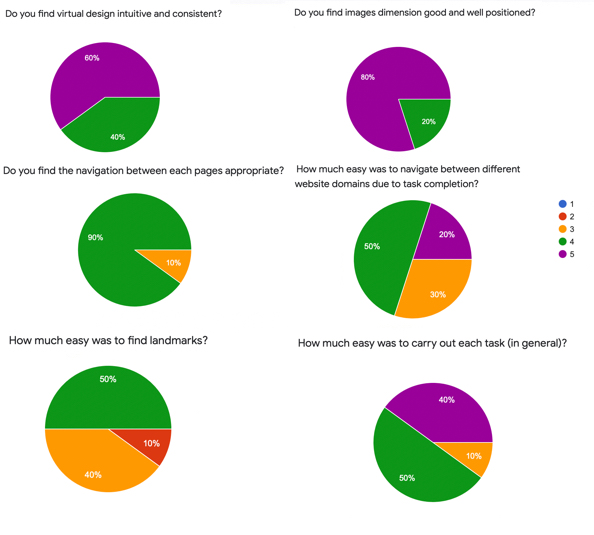
\includegraphics[scale=0.75]{images/questions.jpg}}
    \caption{Pie charts for each question of the form.}

\end{figure}


\subsection{Comment}
As evidenced by the results obtained from the study carried out, the two tester profiles used for the study gave the expected results. The testers belonging to Profile 2, older and with a background skilled from the point of view of the IT sector, gave values of time and errors higher than the testers of profile 1 even if they managed enough to complete the tasks to which they were subjected and expressing high values of appreciation for the site, which demonstrates that, although the system is geared towards sectoral users, the minimalist design and clarity of content displayed works well on a wide range of visitors.



